\let\negmedspace\undefined
\let\negthickspace\undefined
\documentclass[journal,12pt,twocolumn]{IEEEtran}
\usepackage{cite}
\usepackage{amsmath,amssymb,amsfonts,amsthm}
\usepackage{algorithmic}
\usepackage{graphicx}
\usepackage{textcomp}
\usepackage{xcolor}
\usepackage{txfonts}
\usepackage{listings}
\usepackage{enumitem}
\usepackage{mathtools}
\usepackage{gensymb}
\usepackage{comment}
\usepackage[breaklinks=true]{hyperref}
\usepackage{tkz-euclide} 
\usepackage{listings}
\usepackage{gvv}                                        
\def\inputGnumericTable{}                                 
\usepackage[latin1]{inputenc}                                
\usepackage{color}                                            
\usepackage{array}                                            
\usepackage{longtable}                                       
\usepackage{calc}                                             
\usepackage{multirow}                                         
\usepackage{hhline}                                           
\usepackage{ifthen}                                           
\usepackage{lscape}

\newtheorem{theorem}{Theorem}[section]
\newtheorem{problem}{Problem}
\newtheorem{proposition}{Proposition}[section]
\newtheorem{lemma}{Lemma}[section]
\newtheorem{corollary}[theorem]{Corollary}
\newtheorem{example}{Example}[section]
\newtheorem{definition}[problem]{Definition}
\newcommand{\BEQA}{\begin{eqnarray}}
\newcommand{\EEQA}{\end{eqnarray}}
\newcommand{\define}{\stackrel{\triangle}{=}}
\theoremstyle{remark}
\newtheorem{rem}{Remark}
\begin{document}
\bibliographystyle{IEEEtran}
\vspace{3cm}
\title{10.5.3}
\author{EE23BTECH11027 - K RAHUL$^{*}$% <-this % stops a space
}
\maketitle
\newpage
\bigskip
\renewcommand{\thefigure}{\theenumi}
\renewcommand{\thetable}{\theenumi}
\section{Question:}
\subsection{Question statement}
The first and the last terms of an AP are 17 and 350 respectively. If the common difference
is 9, how many terms are there and what is their sum?
\subsection{Solution}
The expression to find the $n^{th}$ term of the Arithmetic Progression is given by
\begin{table}[h]
\setlength{\arrayrulewidth}{0.3mm}
\setlength{\tabcolsep}{15pt}
\renewcommand{\arraystretch}{1.5}

table 1\\

\begin{tabular}{ |p{1cm}|p{3cm}|p{1cm}| }
\hline
\multicolumn{3}{|c|}{Parameters in expression}\\
\hline
Symbol & Description & Value\\
\hline
n & The nth term of series & To be computed\\
\hline
$a_n$ & nth term of series & 350\\
\hline
$a_0$ & 0th term of series & 17 \\
\hline
d & Common difference of AP & 9\\
\hline
\end{tabular}


\end{table}
\bigskip
\begin{align}\label{eq:1}a_n = a_0 + nd\end{align}
The question asked for the number of terms present in the AP, hence from \ref{eq:1}
\begin{align}\label{eq:2} n=\frac{a_n-a_0}{d} \end{align}
Thus, plugging the values into equation \ref{eq:2} 
$$\fbox{n = 37}$$
Now, the expression for sum of numbers in an Arithmetic Progression is given by
\begin{equation}\label{eq:3} S_n = (\frac{n+1}{2})(a_1+a_n)\end{equation}
Where $S_n$ is the sum of n+1 terms of AP and the rest of the symbols carry the same meaning as mentioned above.\\
Plugging the values into equation, we get
$$S_n = 6973$$\\\\
Thus, the number of terms present in the Arithmetic Progression is 38 and sum of terms of the Arithmetic Progression is 6973.
\section{Question 2}
\subsection{Question statement}
Express nth term as x(n) in terms of u(n) and find it's Z transform. Additionally, plot the graph of x(n) using python and give the ROC of X(Z).\\
\subsection{Solution}
The formula for sum of numbers in an AP is 
$$a_n = a_0 + nd$$
\begin{table}[h]
\setlength{\arrayrulewidth}{0.3mm}
\setlength{\tabcolsep}{15pt}
\renewcommand{\arraystretch}{1.5}

table 1\\

\begin{tabular}{ |p{1cm}|p{3cm}|p{1cm}| }
\hline
\multicolumn{3}{|c|}{Parameters in expression}\\
\hline
Symbol & Description & Value\\
\hline
n & The nth term of series & N/A\\
\hline
$a_n$ & nth term of series & To be computed\\
\hline
$a_0$ & 0th term of series & 17 \\
\hline
d & Common difference of AP & 9\\
\hline
\end{tabular}

\end{table}
\bigskip
Thus, plugging the values as given in the question
\begin{equation}\label{eq:1st}a_n = 8+9n\end{equation}
Now, the function x(n) is in terms of u(n) as well.\\ Thus from equation \ref{eq:1st},
\begin{equation}\label{eq:2nd}x(n) = (8 + 9n)u(n)\end{equation}
where u(n) is the unit step function\\
Now, it's Z transform has to be computed.
The Z transform for a general function f(n) is calculated by using the expression
\begin{equation}\label{Z Transform}X(Z) = \mathcal{Z}(x|n|) = \sum^{\infty}_{n=-\infty}x[n]Z^{-n}\end{equation}
Where
\begin{itemize}
    \item X(Z) is the function as asked in the question.
    \item $\mathcal{Z}(x|n|)$ is the Z transform.
    \item x[n] is the value of the function defined in equation \ref{eq:2nd} at a value n.
\end{itemize}
\newpage
Now, plugging in the function defined in equation \ref{eq:2nd} into expression \ref{Z Transform}, we get
\begin{equation}\label{7} X(Z) = \sum^{\infty}_{n=0}(8+9n)Z^{-n}\end{equation}
Now, this expression can be evaluated only when $|Z|>1$(Thus, making $|Z|>1$ the region of convergence).\\
If $|Z|>1$, then expression \ref{7} simplifies to
\begin{equation}\label{8}X(Z) = (8-5Z)({(1-Z)}^{-2}\end{equation}
\newpage
\begin{flushleft}
\begin{figure}[h]
\renewcommand\thefigure{1}
    \caption{Enter Caption}
    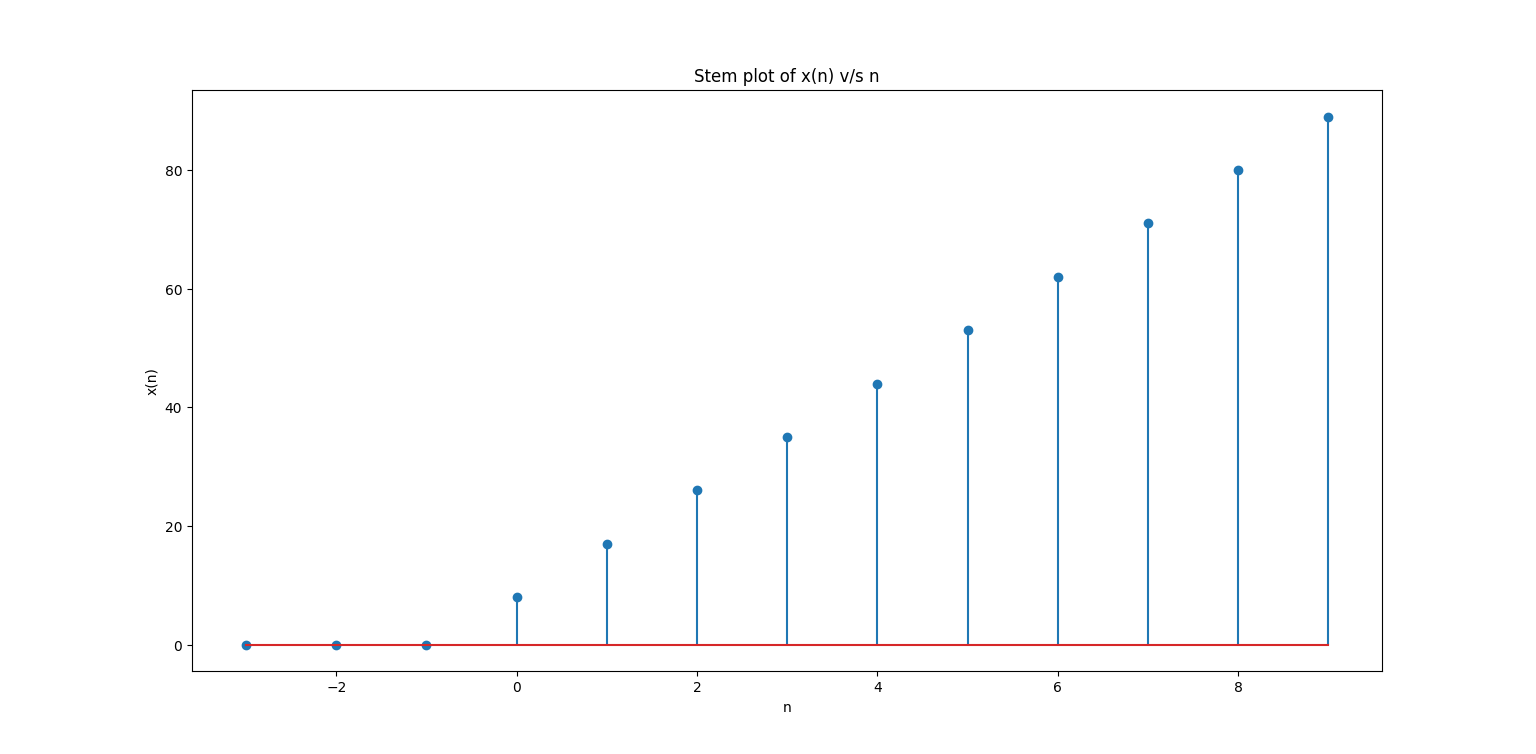
\includegraphics[width=1.1\textwidth]{figs/x(n)_plot.png}
    \label{fig:stem-plot}
\end{figure}
\end{flushleft}

\end{document}
